\documentclass{article}
\usepackage[utf8]{inputenc}
\usepackage{graphicx}

\title{320 Requirements}
\author{Trevor's Team}
\date{\today}

\begin{document}
\begin{titlepage}

\maketitle

\begin{abstract}
\textbf{Purpose of System:} \newline
\newline
The purpose of this system is to be an online tutor for students at the University of Massachusetts Amherst. This learning tool would help teach the students and allow them to create ER diagrams and submit them as homework assignments. They can then be graded by solutions uploaded by the instructor of a course. Feedback will then be provided to help the student learn from their mistakes. The benefits of this system is that it makes submitting learning in the course and submitting homework much easier for both the students and instructor. \newline


\textbf{Scope:}
\newline \newline
This document will clearly outline the requirements and the system requirements of ER Diagram Tutoring System. This document should cover all key concepts and fundamental requirements. The requirements should satisfy the standards of the client and provide accuracy in the functionality of the system. 


\end{abstract}

\end{titlepage}

\tableofcontents
\newpage
\begin{section}{Data Dictionary}
\begin{center}
    \begin{tabular}{ | l | l | l |l| p{5cm} |}
   \hline
    Student Info & Pay Info & New Class & Class Availability \\ \hline

    

    
    - Name          &  - Student ID &  - Student ID           & - Student ID  \\
    - Student ID    &  - Amount     &  - Transcript           & - Class ID  \\ 
    - SSN           &  - Name       &  - Section              & - Seat Availability\\ 
    - Date of Birth &  - Address    &  - Discussion Section   & - Class Capacity   \\ 
    - Address       &  - Phone      &  - Class ID             &   \\ 
    - Telp. Number  &  - EMail      &  - Professor            &   \\ 
    - Gender        &               &                         &   \\ 
    - Email         &               &                         &   \\ 
    - Classes Taken &               &                         &   \\ 
    - Grades        &               &                         &\\ \hline

    
       
    
Proof of Registration & Send Payment Due & Billing Info & Class Roster\\ \hline
       - Student ID   &  - Student ID    &  - Student ID& - Student ID  \\ 
       - Day          &  - Name          &  - Name      & -Name\\
       - Time         &  - Amount        &  - Address   & Major   \\ 
       - Room         &  - Receipt ID    &  - Phone     &   \\ 
       - Class ID     &                  &    - Email   & \\ 
                      &                  &    - Amount  & \\
                      &                  &              &   \\ 
                      &                  &               &\\ \hline
    
    
    
    
    
    
    
    
    
    \hline
    \end{tabular}
\end{center}
\end{section}
\newpage

\begin{section}{Context Level Diagram}
    \begin{figure}[h!]
        \begin{center}
           \centerline{ 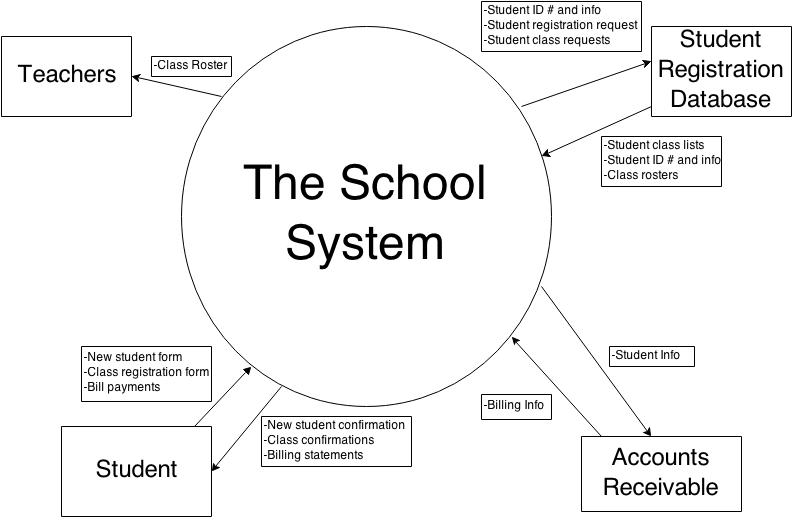
\includegraphics[height=13cm]{DF.jpg}}
            \caption{DFD Context Diagram}
        \end{center}
    \end{figure}
\end{section}
\newpage
\begin{section}{Level 0 Diagram}
    \begin{figure}[h!]
        \begin{center}
            \centerline{\includegraphics[height=13cm]{DFD Level0.jpg}}
            \caption{DFD Level 0 Diagram}
        \end{center}
    \end{figure}
\end{section}
\newpage
\begin{section}{Functional Requirements}

    \begin{subsection}{Allow Student to Draw a Diagram}
    Primary Actor: Student \newline
    Precondition: Student is logged in and viewing a            question \newline
    Trigger: Student chooses a question to work on \newline
    Success end condition: Student can submit answer            \newline
    Failed end condition: Diagram is not drawn \newline
    \newline
    Steps:
    \begin{enumerate}
    \item{Empty space available to draw diagram}
    \item{Student picks a diagram type (Chen’s/Crow’s Foot)}
    \item{Student picks shapes from toolbox and places in           diagram}
    \item{Student places text inside shapes}
    \item{Student places links between shapes}
    \item{Student can edit or remove anything already placed on the diagram before finalizing}
    \end{enumerate}
    Exceptions:
    \begin{enumerate}
    \item{Teacher draws diagram that students must edit             \newline
        *Draw space will not be empty, student will be able to           make changes to present diagram}
    \end{enumerate}
    \end{subsection}
    
    \begin{subsection}{Submit Answer}
    Primary Actor:Student \newline
    Precondition: Student is ready to submit answer \newline
    Trigger: Pressing the submit button \newline
    Success end condition: Feedback and/or grade is given       \newline
    Failed end condition: Nothing is given back to student      \newline
    \newline
    Steps:
    \begin{enumerate}
    \item{Student submits answer by pressing the submit             button}
    \item{System processes answer and decides validity}
    \item{Outputs feedback and/or grade for student to see}
    \item{Answer is saved into database}
    \end{enumerate}
    Exceptions:
    \begin{enumerate}
    \item{Student leaves area blank \newline
	*Answer is just marked as wrong}
	\addtocounter{enumi}{1}
    \item{Teacher never properly input the correct answer or     feedback \newline
	*Student is told that there's nothing to report}
    \end{enumerate}
    \end{subsection}
    
    \begin{subsection}{Allow Teacher to Create    Questions/Feedback}
    
    Primary Actor: Teacher \newline
    Precondition: Teacher is logged in a specific course. \newline
    Trigger: Teacher selects a specific Homework to create a     question. \newline
    Success end condition: Question is uploaded and the instructor is able to see it. \newline
    Failed end condition: Students don’t see the question       properly. \newline
    \newline
    Steps:
    \begin{enumerate}
    \item{Teacher clicks on a “create” button to create the           question.}
    \item{Teacher select the number of the question that             he/she wants to post for a previously chosen               homework.}
    \item{Teacher writes the database schema of the ER              diagram that is going to be drawn by the student, in         an available textbox.}
    \item{Teacher provides a general feedback in a textbox            provided.}
    \item{Teacher clicks on a “add” button to add the                 question of the homework.}
    \item{Teacher clicks on a “preview” button to see the           students point of view of the entire homework.}
    \item{Teacher clicks on a “submit” button to submit the           entire homework.}
    \end{enumerate}
    Exceptions:
    \begin{enumerate}
    \item{Teacher tries to create question but he/she doesn't have Internet connection.}
    \end{enumerate}
    \end{subsection}
    
    \begin{subsection}{Select Question to Answer}
    Primary Actor: Student \newline
    Precondition: Student is logged in and is in an assignment         \newline
    Trigger: The student attempts to select a new question      to attempt to answer \newline
    Success End Condition: Question that the student selects     successfully loads \newline
    Failed End Condition: The question that is selected does     not load \newline
    \newline
    Steps:
    \begin{enumerate}
    \item{Student scrolls through the list of questions in the assignment.}
    \item{Student selects the question they would like to        answer from the list.}
    \item{Webpage for the selected question loads}
    \item{Student can read and answer question}
    \end{enumerate}
    Exceptions: None
    \end{subsection}

\end{section}

\begin{section}{Environmental Requirements}

    \begin{subsection}{ToolBox for Drawing Diagram}
    A ToolBox will help the student draw the diagram. The student will first select whether he wants to draw a Chen’s Diagram or a Crow’s Foot Diagram. The toolbox will then adjust accordingly, displaying the shapes and edges that are common to the chosen diagram. This will include squares, circles, directed edges, and tick marks (for Crow’s Foot).
    
    \end{subsection}
    
    \begin{subsection}{Save Progress of Current Assignment}
    When a student logs in, he/she should be able to start a quiz. As the student progresses through the quiz, the answers answered by the student should be saved in the students personal database. In that way, if he/she wants to stop and continue with the quiz other time, he can do so without starting all over again.
    \end{subsection}
    
    \begin{subsection}{List of Available Questions and Their Status}
    While a student is answering questions, there will be a list of all the questions listed horizontally at the top of the page.  Next to each question number will be a small image.  The image will either be a green check mark if the question is answered correctly, a red x is the question is answered incorrectly or a black question mark if the question has not been answered yet.  When the status of the question changes then so will the image next to the question number.
    \end{subsection}
    
    \begin{subsection}{Open Space to Draw Diagram}
    After a student selects which question they want to work on a white drawing space will be given to them in which to draw their answer. Off to the side of this space will be the toolbox which they use to do the drawing. There will also be a submit button off to the side somewhere which is what the student is to press when they're finished with their answer.
    \end{subsection}
    
    \begin{subsection}{Compatibility With Multiple Browsers}
    The program will open and be usable with all major internet browsers. Including Safari, Chrome, Firefox, Internet Explorer.
    \end{subsection}

\end{section}

\begin{section}{Performance Requirements}

    \begin{subsection}{Correctness Analysis}
    The ER diagram drawn by the student generates a database schema that will be compared with schema provided by the professor in the question. If they are equal, then the solution provided by the student is correct, otherwise is wrong. This should be done in a matter of seconds.
    \end{subsection}
    
    \begin{subsection}{Question Loading}
    When the student selects a new question to attempt to answer the question should load within 5 seconds when the server is not busy and should load within 10 seconds when the server is busy.
    \end{subsection}
    
\end{section}

\begin{section}{Safety/Security Requirements}

    \begin{subsection}{Student Navigates to the Main Page}
    Description: The student reaches the main page of an assignment. \newline
Primary Actor: Student \newline
Secondary Actor: Content author \newline
Steps:
\begin{enumerate}
\item{The page loads, displaying the correct questions for the assignment selected.}
\item{All questions load and display properly.}
\item{The student response areas load and allow for proper student input.}
\end{enumerate}
Successful Post Conditions:
\begin{itemize}
\item{The page displayed is for the correct class and assignment.}
\item{The student gains no access to non-student interfaces.}
\item{The submission of answers writes only to the students record for the assignment.}
\end{itemize}
Exceptional Condition:
\begin{itemize}
\item {The student attempts to access a page he/she should not have access to - the student is displayed an appropriate warning message and is not given access to any assignment or interface that he/she is not meant to have access to.}
\end{itemize}

\end{subsection}

   \begin{subsection}{Professor Navigates to the Main Page}
   Description: The professor reaches the main page of an assignment. \newline
Primary Actor: Professor \newline
Secondary Actor: Content author \newline
Steps:
\begin{enumerate}
\item{The page loads, displaying the tools for adding or modifying an assignment and the information corresponding to student-submitted scores.}
\item{All questions load and display properly.}
\item{The content-create pallet allows for the full range of content creation.}
\item{The data corresponding to student submissions accurately reflects the data currently stored for each student.}
\end{enumerate}
Successful Post Conditions:
\begin{itemize}
\item{The page that is displayed shows the correct class and assignment.}
\item{The professor is shown the assignment creation and management page.}
\item{The content changes that are made only apply to the currently selected assignment.}
\end{itemize}
Exceptional Condition:
\begin{itemize}
\item{The professor attempts to access a page he/she should not have access to - the professor is displayed an appropriate warning message and is not given access to any assignment or interface he/she is not meant to have access to.}
\end{itemize}
\end{subsection}

\begin{subsection}{Student Closes Application With Unsaved Answers in the Window}
Description: The student has entered a response to a question without saving or submitting the assignment. \newline
Primary Actor: Student \newline
Secondary Actor: Professor \newline
Steps:
\begin{enumerate}
\item{The student enters a full or partial response to an assignment question.}
\item{The student does not save or submit the assignment.}
\item{The student closes the assignment page.}
\end{enumerate}
Successful Post Condition:
\begin{itemize}
\item{The student is shown a prompt asking if he/she is sure about wanting to leave the page with unsaved responses.}
\end{itemize}
\end{subsection}

\begin{subsection}{Student Submits Page with Blank Answers}
Description: The student submits an assignment with a response that was left blank. \newline
Primary Actor: Student \newline
Secondary Actor: Professor \newline
Steps:
\begin{enumerate}
\item{The student accesses the page.}
\item{The student inputs and saves responses to some questions.}
\item{The student submits the assignment with some responses that are left entirely blank.}
\end{enumerate}
Successful Post Condition:
\begin{itemize}
\item{The student is presented with a prompt asking he/she is sure about wanting to submit a blank response to a question.}
\end{itemize}

\end{subsection}

\begin{subsection}{Student Submits Assignment That Was Already Submitted}
Description: After a student submits an assignment, he/she tries to submit the same assignment again. \newline
Primary Actor: Student \newline
Secondary Actor: Professor \newline
Steps:
\begin{enumerate}
\item{The student completes an assignment.}
\item{The student completes the same assignment with different answers.}
\item{The student submits the assignment again.}
\end{enumerate}
Successful Post Condition:
\begin{itemize}
\item{The student is presented with a prompt asking if the/she wants to overwrite the submitted assignment - assuming this occurs before the assignment is closed.} 
\end{itemize}
Exceptional Condition:
\begin{itemize}
\item{If the submission comes after the assignment is closed, the student is informed that the assignment is closed and no subsequent submissions are allowed.} 
\end{itemize}
\end{subsection}

\begin{subsection}{Student or Professor Tries to Log Into Someone Else’s Account}
Description: The student or professor tries to log into the  system with the NetID of another student or professor. \newline
Primary Actors: Student, Professor \newline
Secondary Actor: System \newline
Steps:
\begin{enumerate}
\item{The student or professor enters someone else’s NetID into the system.}
\item{The student or professor enters a fake password into the system.}
\item{The student or professor clicks the “Login” button or the enter key.}
\end{enumerate}
Successful Post Conditions:
\begin{itemize}
\item{The system prohibits the student or professor from logging into the system with a NetID and password that do not match.}
\item{The system sends a reply that says that the login was unsuccessful.}
\item{The system prompts the user to try entering a username and password again.}
\end{itemize}
\end{subsection}

\end{section}
%%%%%%%%%%%%%%%%%%%%%%%%%%%%%%%%%
\begin{section}{Robustness Use Cases}
    \begin{subsection}{Student Enters Diagram}
     
    Description: The student submits a diagram in either Chen or CF that is correct but is not the same as the instructor’s.\\
    Primary Actors: Student, System\\
    Secondary Actor: Professor\\
    Steps:
    \begin{enumerate}
    \item The student enters a diagram into the system.
    \item The system checks the diagram against the professor-submitted diagram(s).
    \end{enumerate}
    
     Successful Post Condition: 
    The system marks the student correct.\\
    Exceptional Conditions:
        \begin{itemize}
            \item The student is unable to submit a diagram as an answer to a question.
            \item The system cannot process the student’s submitted diagram so that it can be compared to the professor’s uploaded answer.
            \item The system cannot send the student a response that says if his/her diagram was correct or incorrect.
            \end{itemize}
    \end{subsection}
    
    \begin{subsection}{Student Enters Variant of Incorrect Diagram}
    Description: The student submits a diagram in either Chen or CF that is incorrect.\\
    Primary Actors: Student, System
    Secondary Actor: Professor\\
    Steps:	
    \begin{enumerate}
    \item The student enters a diagram into the system.
    \item The system checks the diagram against the professor-submitted diagram(s).
    \end{enumerate}
    Successful Post Condition: 
        \begin{itemize}
            \item The system marks the student incorrect.
        \end{itemize}
    Exceptional Conditions:
        \begin{itemize}
            \item The student is unable to submit a diagram as an answer to a question.
            \item The system cannot process the student’s submitted diagram so that it can be compared to the professor’s uploaded answer.
            \item The system cannot send the student a response that says if his/her diagram was correct or incorrect.
        \end{itemize}
    \end{subsection}
    \begin{subsection}{Professor or Content}
        Author enters unspecified answer format\\
        Description: The professor or content author enters an answer into the system without specifying a format.\\
        Primary Actor: Professor (or Content Author)\\
        Secondary Actor: System\\
        Steps:	
        \begin{enumerate}
            \item The professor submits an answer into the system.	
            \item The system recognizes that the professor did not submit an answer format.
        \end{enumerate}
            Successful Post Condition: 
                \begin{itemize}
                    \item The system sends a prompt to the professor specifying that the answer was not recorded in the system and that he/she must submit an answer format.
                \end{itemize}
    \end{subsection}
    \begin{subsection}{System Should Never Crash}
    
    Description: Nothing the student does should crash the browser. The system may not respond or react correctly, but it will not crash the students browser or machine.
    \end{subsection}
    \begin{subsection}{ UI Should React Correctly To Student and Professor Actions}
    
    Description: The UI should correctly react to what the student and professor’s actions command.\\
    Primary Actor: Student, Professor\\
    Secondary Actor: System\\
    Steps:
        \begin{enumerate}
            \item The student or professor clicks buttons/links or drags items from a template to the answer submission.
            \item The system follows the links or correctly places the dragged items in the submission box.
            \end{enumerate}
    Successful Post Condition: 
        \begin{itemize}
            \item The system view refreshes so that the student or professor sees his/her actions take place in real time.
        \end{itemize}
    Exceptional Condition:
        \begin{itemize}
            \item A specific student or professor action was not accounted for when the UI was created - the UI does not have the ability to make a response to that action.
        \end{itemize}
    \end{subsection}
    
\end{section}

%%%%%%%%%%%%%%%%%%%%%%%%%%%%%%%%%%%%%%%%%%%%%%%%%%%%%%%%%%%%%%%%%%%%%%%%%%%%%%%%%


\begin{section}{Accuracy Requirements}

\begin{subsection}{Student Submits Correct Diagram}
Description: The student answers a question by submitting the correct diagram. \newline
Primary Actors: Student, System \newline
Secondary Actor: Professor \newline
Steps:
\begin{enumerate}
\item{The student enters a diagram as an answer to a question.}
\item{The system compares that diagram to the correct diagram that was uploaded by the professor.}
\item{The system recognizes that the diagram submitted matches the diagram that was uploaded by the professor.}
\end{enumerate}
Successful Post Condition:
\begin{itemize}
\item{The system marks the student’s answer to the question as correct.} 
\end{itemize}
Exceptional Conditions:
\begin{itemize}
\item{The student is unable to submit a diagram as an answer to a question.}
\item{The system cannot process the student’s submitted diagram so that it can be compared to the professor’s uploaded answer.}
\item{The system cannot send the student a response that says if his/her diagram was correct or incorrect.}
\end{itemize}
\end{subsection}

\begin{subsection}{Student Submits Incorrect Diagram}
Description: The student answers a question by submitting an incorrect diagram. \newline
Primary Actors: Student, System \newline
Secondary Actor: Professor \newline
Steps:
\begin{enumerate}
\item{The student enters a diagram as an answer to a question.}
\item{The system compares that diagram to the correct diagram that was uploaded by the professor.}
\item{The system recognizes that the diagram submitted matches the diagram that was uploaded by the professor.}
\end{enumerate}
Successful Post Condition:
\begin{itemize}
\item{The system marks the student’s answer to the question as incorrect.}
\end{itemize}
Exceptional Conditions:
\begin{itemize}
\item{The student is unable to submit a diagram as an answer to a question.}
\item{The system cannot process the student’s submitted diagram so that it can be compared to the professor’s uploaded answer.}
\item{The system cannot send the student a response that says if his/her diagram was correct or incorrect.}
\end{itemize}
\end{subsection}

\end{section}



%%%%%%%%%%%%%%%%%%%%%%%%%%%%%%%%%%%%%%%%%%%%%%%%
%%%%%%%%%%%%%%%%%%%%%%%%%%%%%%%%%%%%%%%%%%%%%%%%
\begin{section}{Login/Logout System Use Cases}
%%%%%%%%%%%%%%%%%%%%%%%%%%%%%%%%%%%%%%%%%%%%%%%%
%%%%%%%%%%%%%%%%%%%%%%%%%%%%%%%%%%%%%%%%%%%%%%%%
%%%%%%%%%%%%%%%%%%%%%%%%%%%%%%%%%%%%%%%%%%%%%%%%%%%%%%%%%%%%%%%%%%%%%%%%%%%%%%%%%
    \begin{subsection}{Student or professor correctly logs into the system}
        Description: The student or professor logs into the system with the correct username and password.\\
        Primary Actors: Student, Professor\\
        Secondary Actor: System\\
        Steps:
        \begin{enumerate}
            \item The student or professor enters his/her correct NetID as a username.
            \item The student or professor enters his/her correct password.
            \item The student or professor clicks the “Login” button or the enter key.
        \end{enumerate}
        Successful Post Condition:\\
        \begin{itemize}
        \item The student or professor is successfully logged into his/her account on the system and can see his/her homepage on the screen.\\
        Exceptional Condition:
        \item The system does not recognize that the correctly entered username and password are associated with an existing account.
        \end{itemize}
        \end{subsection}
        %%%%%%%%%%%%%%%%%%%%%%%%%%%%%%%%%%%%%%%%%%%%%%%%%%%%%%%%%%%%%
        \begin{subsection}{Student or professor incorrectly logs into the system}
    Description: The student or professor logs into the system with an incorrect username and/or password.\\
    Primary Actors: Student, Professor\\
    Secondary Actor: System\\
    Steps:
        \begin{enumerate}
            \item The student or professor enters an incorrect NetID as a username.
            	and/or
            \item The student or professor enters an incorrect password.
            \item The student or professor clicks the “Login” button or the enter key.\\
        \end{enumerate}
    Successful Post Conditions:
        \begin{itemize}
            \item The system prohibits the student or professor from logging into the system with a NetID and password that do not match.
            \item The system sends a reply that says that the login was unsuccessful.
            \item The system prompts the user to try entering a username and password again.
        \end{itemize}
    \end{subsection}
%%%%%%%%%%%%%%%%%%%%%%%%%%%%%%%%%%%%%%%%%%%%%%%%%%%%%%%%%%%%%%%%%%%%%%%%%%%%%%%5
    \begin{subsection}{Student or professor correctly logs out of the system}
        Description: The student or professor is able to successfully log out of the system.\\
        Primary Actors: Student, Professor\\
        Secondary Actor: System\\
        Steps:
        \begin{itemize}
            \item The student or professor clicks the “Log Out” button.
            \item Successful Post Condition:
            \item The student or professor receives a reply from the system that says that the log out was successful.
        \end{itemize}
        Exceptional Condition:
        \begin{itemize}
            \item The “Logout” button does not have the functionality to successfully log out the student or professor.
        \end{itemize}
    \end{subsection}
\end{section}



%%%%%%%%%%%%%%%%%%%%%%%%%%%%%%%%%%%%%%%%%%%%%%%%%%%%%%%%%%%%%%%%%%%%%%%%%%%%%%%%%%%%%%%%%%%%
%%%%%%%%%%%%%%%%%%%%%%%%%%%%%%%%%%%%%%%%%%%%%%%%%%%%%%%%%%%%%%%%%%%%%%%%%%%%%%%%%%%%%%%%%%%%





\begin{section}{Professor UI Requirements}

\begin{subsection}{Professor Clicks on Side or Top Navigation Buttons}
Description: While on any page containing navigation links in the side or top bars, the professor clicks on a nav link \newline
Primary Actors: Professor \newline
Steps:
\begin{enumerate}
\item{The professor is logged into any of the main pages containing nav links}
\item{The professor clicks on any link}
\end{enumerate}
Successful Post Conditions:
\begin{itemize}
\item{The professor is directed to the page intended by the link}
\end{itemize}
Exceptional Condition:
\begin{itemize}
\item{The professor is already on the page of the link they are clicking - nothing happens and the page does not change.}
\end{itemize}
\end{subsection}

\begin{subsection}{Professor Clicks on the Assignment Submission Ticker}

Description: From the main landing page the professor clicks on the assignment submission ticker \newline 
Primary Actor: Professor \newline
Steps:
\begin{enumerate}
\item{The professor is on the main page after login}
\item{The professor clicks on the Assignment Submission Ticker Pane}
\end{enumerate}
Successful Post Condition:
\begin{itemize}
\item{The professor is redirected to a larger detailed view with a time directed log of student submission stats for assignments the professor has created, or is linked to through class ownership}
\end{itemize}
Exceptional Post Condition:
\begin{itemize}
\item{The professor has no submissions in his feed - he is directed to the log but is not shown any information}
\end{itemize}
\end{subsection}

\begin{subsection}{Professor Clicks on the Class or Student Ticker}
Description: From the main landing page the professor clicks on enrolled student/ class ticker pane \newline
Primary Actor: Professor \newline
Steps:
\begin{enumerate}
\item{The professor is on the main page after login}
\item{The professor clicks on the enrolled student/ class ticker pane}
\end{enumerate}
Successful Post Condition:
\begin{itemize}
\item The professor is redirected to a larger detailed view with the option to sort by class or student name to display stats pertaining to course enrollment and individual student assignment histories
\end{itemize}
\end{subsection}

\begin{subsection}{Professor Clicks to Expand the Assignment Creation Sandbox}
Primary Actor: Professor \newline
Steps:
\begin{enumerate}
\item{The professor is on the main page after login} 
\item{The professor clicks to expand the assignment creation sandbox}
\end{enumerate}
Successful Post Condition:
\begin{itemize}
\item{The professor is taken to the assignment creation page and any potential diagrams or questions created in the sandbox are stored and transferred to the assignment creation window}
\end{itemize}
\end{subsection}

\newpage

\begin{subsection}{Professor View}
\begin{figure}[h!]
        \centerline{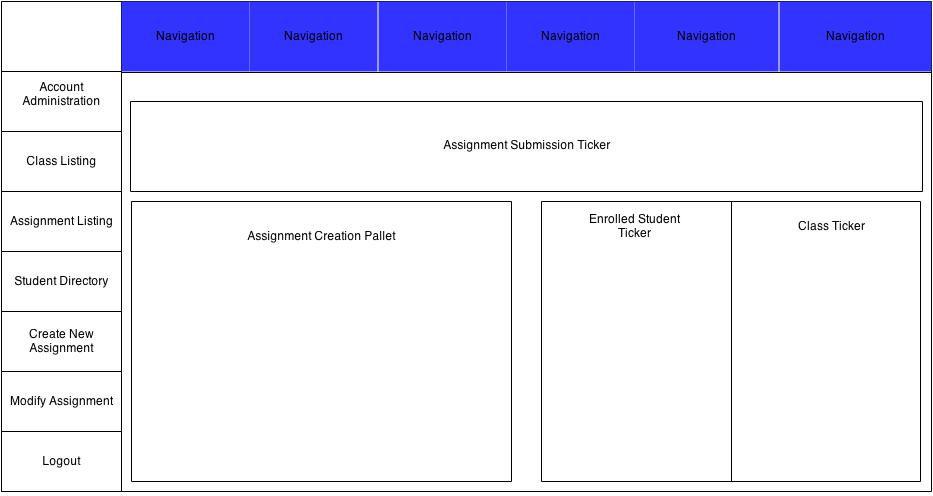
\includegraphics[width=17cm]{ProfessorView.jpg}}
        \caption{Professor's User Interface}
\end{figure}
\end{subsection}
\newpage

\begin{subsection}{Create}
\begin{figure}[h!]
        \centerline{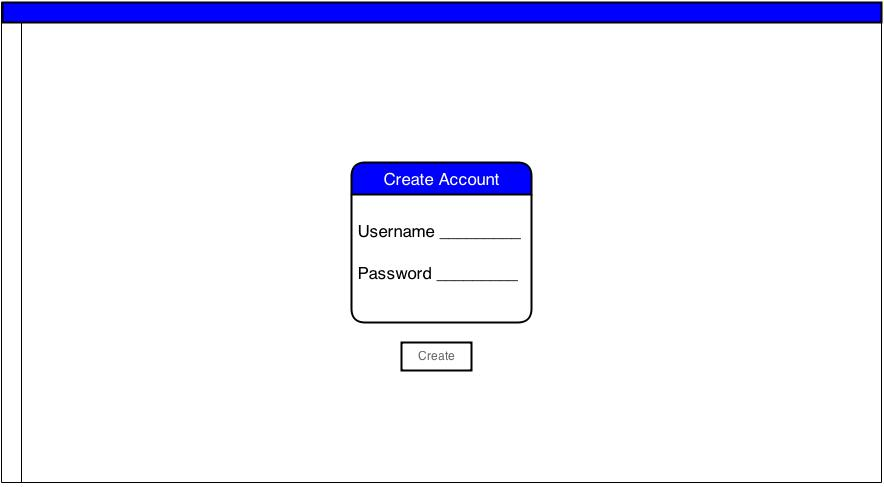
\includegraphics[width=17cm]{UICreate.jpg}}
        \caption{User Interface to create question}
\end{figure}
\end{subsection}
\newpage
\begin{subsection}{Login}
\begin{figure}[h!]
        \centerline{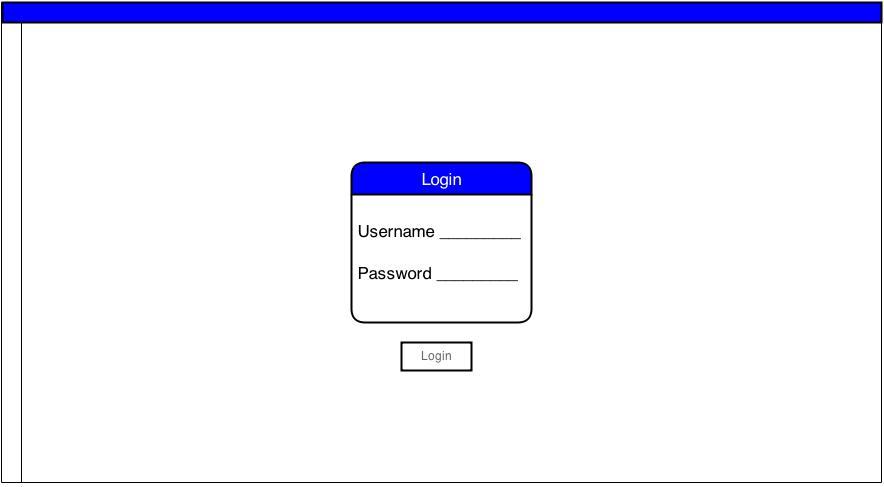
\includegraphics[width=17cm]{UILogin.jpg}}
        \caption{Login User Interface}
\end{figure}
\end{subsection}
\newpage
\begin{subsection}{Student}
\begin{figure}[h!]
        \centerline{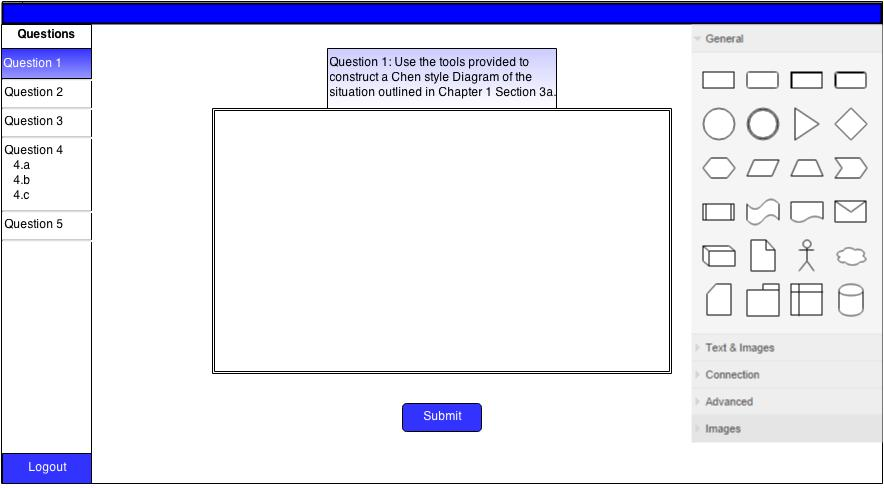
\includegraphics[width=17cm]{uistudent.jpg}}
        \caption{User Interface for the student}
\end{figure}
\end{subsection}


\end{section}















\end{document}
